\section{Simulations}

%---------------------------------------------------

\begin{frame}{\textit{PE Model}: Simulation Process}
	
	Given the model selection, the following process is performed:
	
	\begin{enumerate}
		\item Selection of constants and initial conditions
		\item Discretization method (RK4)
		\item Plotting
	\end{enumerate}
\end{frame}

%---------------------------------------------------
\begin{frame}[fragile]
		
	\frametitle{\textit{PE Model}: Selection of Constants}
		    
	\begin{python}
		vetor_a = [1, 1, 3]
		vetor_b = [
			0.5 * (vetor_a[0] - vetor_a[1] - vetor_a[2]),
			0.5 * (vetor_a[1] - vetor_a[2] - vetor_a[0]),
			0.5 * (vetor_a[2] - vetor_a[0] - vetor_a[1]),
		]
		c = math.sqrt(3/4)
				
		f_inv = 10800
		vetor_h = [-1, 0, 0]
		vetor_f = [0.1, 0, 0]
		g_0 = 8
		kappa_0 = 1 / 48
		nu_0 = kappa_0
	\end{python}
\end{frame}

%---------------------------------------------------

\begin{frame}{\textit{RK4 Discretization Method}: General Characteristics}
	
	A method is explicit Runge-Kutta of order $4$ if and only if it satisfies three properties:
	\begin{enumerate}
		\item Explicit single-step method;
		\item It presents good stability for ordinary differential equations (ODEs).
		\item It has a global error of the order of $\mathcal{O}(h^4)$, ensuring high accuracy with a moderate computational cost.
	\end{enumerate}
\end{frame}

%---------------------------------------------------

\begin{frame}{\textit{RK4 Discretization Method}: Formulation}
	
	Taking \cite{roma2023} as a reference, we can express the RK44 method as follows:
	\begin{equation*}
		\Phi(t,y,h) = \frac{1}{6} \left( \kappa_1 + 2\kappa_2 + 2\kappa_3 + \kappa_4 \right) \quad \text{com} \quad
		\begin{cases}
			\kappa_1 = f(t,y)                                       \\
			\kappa_2 = f \left( t + h/2, y + (h/2) \kappa_1 \right) \\
			\kappa_3 = f \left( t + h/2, y + (h/2) \kappa_2 \right) \\
			\kappa_4 = f \left( t + h, y + h\kappa_3 \right)        
		\end{cases}
	\end{equation*}
\end{frame}

%---------------------------------------------------
\begin{frame}[fragile]
		
	\frametitle{\textit{PE Model}: Initial conditions - default}
	The first initial condition is the one given by default and is intended to reproduce figure 1 of the article.   
	\begin{python}
# Initial conditions
x0 = [0.1, 0, 0]
y0 = [0.1, 0, 0]
z0 = [0.1, 0, 0]
	\end{python}
\end{frame}

%---------------------------------------------------

\begin{frame}{\textit{PE Model}: Results for Standard Initial Condition}
	\begin{figure}
		\centering
		\begin{subfigure}[b]{0.45\textwidth}
			\centering
			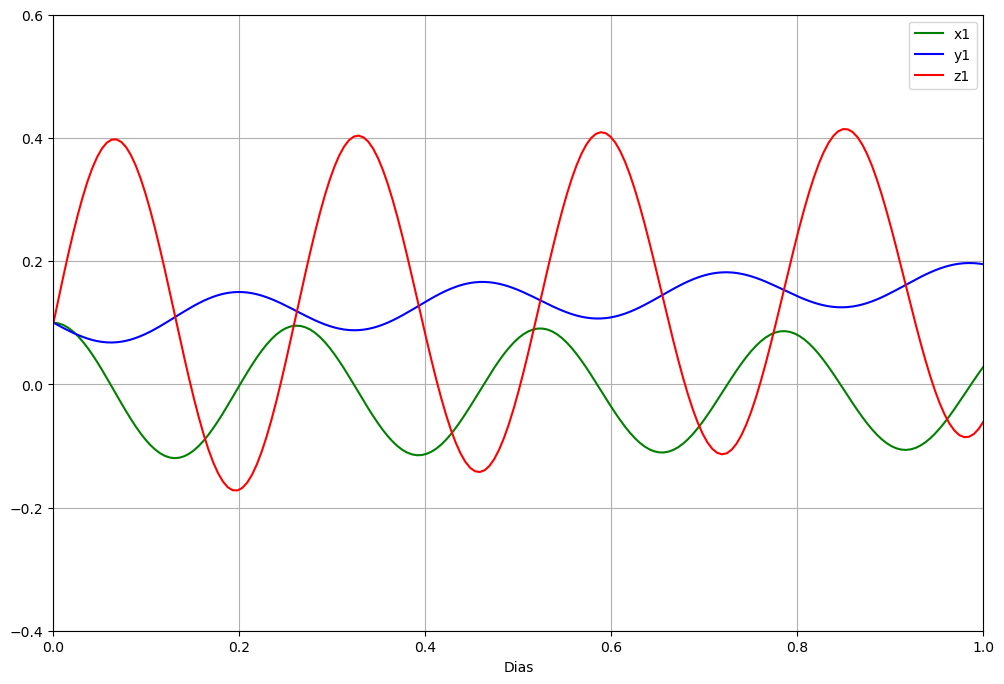
\includegraphics[width=\textwidth]{img/p01d01.png}
			\caption{Standard condition - 01 day\\(reproduction)}
			\label{fig:p01d01}
		\end{subfigure}
		\hfill
		\begin{subfigure}[b]{0.45\textwidth}
			\centering
			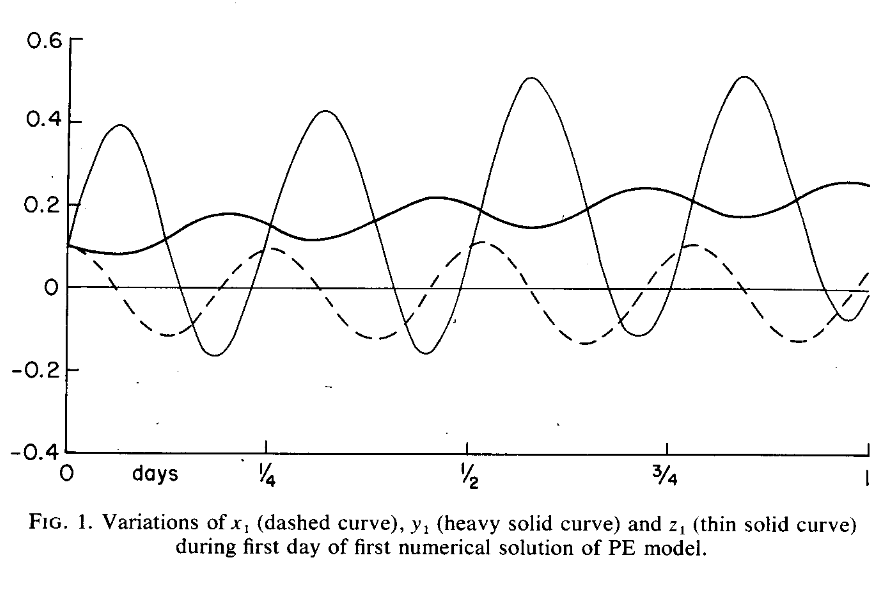
\includegraphics[width=\textwidth]{img/p01d01rel.png}
			\caption{Standard condition - 01 day\\(article)}
			\label{fig:p01d01rel}
		\end{subfigure}
	\end{figure}
\end{frame}

%---------------------------------------------------

\begin{frame}{\textit{PE Model}: Results for Standard Initial Condition}
	\begin{figure}
		\centering
		\begin{subfigure}[b]{0.45\textwidth}
			\centering
			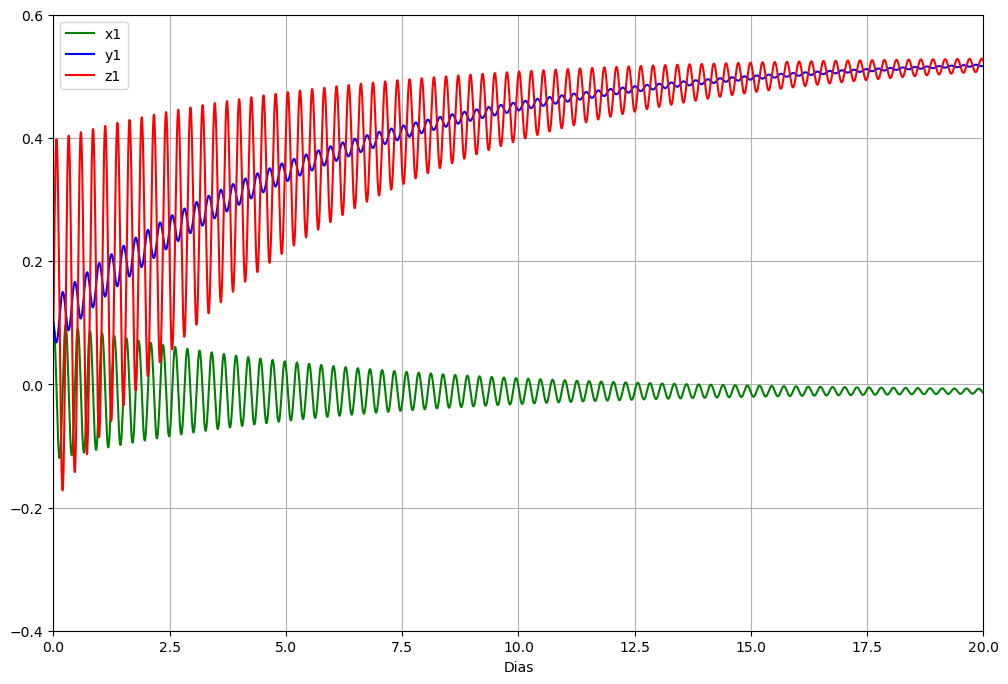
\includegraphics[width=\textwidth]{img/p01d20.png}
			\caption{Standard condition - 20 days}
			\label{fig:p01d20}
		\end{subfigure}
		\hfill
		\begin{subfigure}[b]{0.45\textwidth}
			\centering
			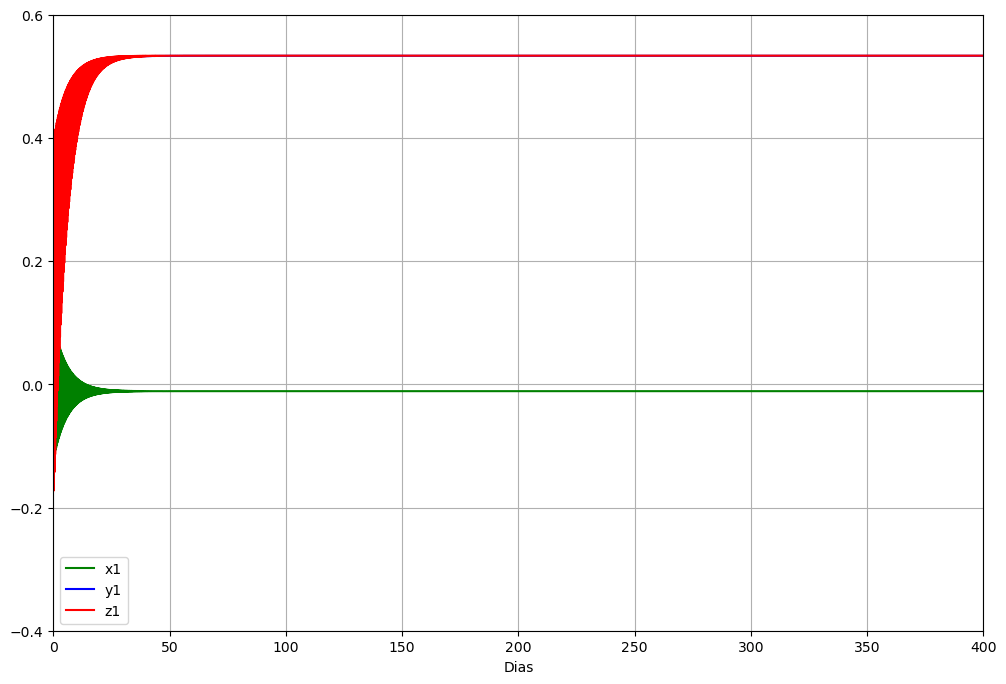
\includegraphics[width=\textwidth]{img/p01d400.png}
			\caption{Standard condition - 400 days}
			\label{fig:p01d400}
		\end{subfigure}
	\end{figure}
\end{frame}



%---------------------------------------------------
\begin{frame}{Hadley Conditions}
	
	The Hadley circulation is a pattern of atmospheric circulation in the tropics, where warm air rises near the equator and descends at higher latitudes, forming a convective cycle.
	\begin{itemize}
		\item In 1735, Hadley incorporated the effect of Earth's rotation, showing that air velocity varies with latitude, influencing the predominant wind direction in the tropics.
		              
		\item It is based on the conservation of angular momentum, ensuring the balance of atmospheric motion and preventing changes in Earth's rotation.
		              
		\item Responsible for the predominant winds in the tropics and the redistribution of heat in the atmosphere, influencing global climate patterns.
	\end{itemize}
\end{frame}

%---------------------------------------------------

\begin{frame}{\textit{PE Model}: Initial Conditions - Hadley 01}
	From the article \cite{gent1982}, we have that the vector values for Hadley conditions are defined as:
	\begin{align*}
		x_1 & = - \nu_0 a_1 y_1,                                                \\
		y_1 & = \frac{F_1}{a_1} v_0 \left( 1 + a_1 g_0 + \nu_0^2 a_1^2 \right), \\
		z_1 & = \left( 1 + \nu_0^2 a_1^2 \right) y_1                            \\
		x_2 & = y_2 = z_2 = x_3 = y_3 = z_3 = 0                                 
	\end{align*}
	
\end{frame}

%---------------------------------------------------

\begin{frame}[fragile]
		
	\frametitle{\textit{PE Model}: Initial Conditions - Hadley 01}
	Adapting to the code, we have:
	
	\begin{python}
# Initial conditions
y1 = (
    vector_f[1]
    / vector_a[1]
    * nu_0
    * (1 + vector_a[1] * g_0 + nu_0**2 * vector_a[1] ** 2)
)
z1 = (1 + nu_0**2 * vector_a[1] ** 2) * y1
x1 = -nu_0 * vector_a[1] * y1

hadley01_initial_x = [x1, 0, 0]
hadley01_initial_y = [y1, -(10 ** (-5)), 0]
hadley01_initial_z = [z1, 10 ** (-5), 0]

	\end{python}
\end{frame}

%---------------------------------------------------

\begin{frame}{\textit{PE Model}: Results for Hadley 01 Condition}
	\begin{figure}
		\centering
		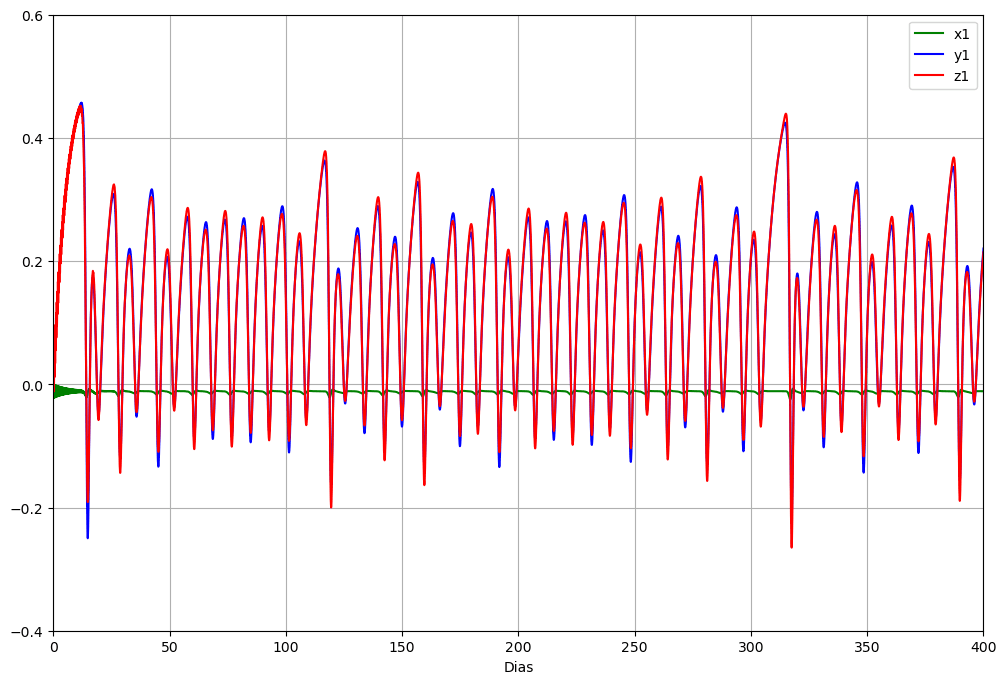
\includegraphics[width=0.5\textwidth]{img/p02d260.png}
		\caption{Hadley 01 - 400 days}
		\label{fig:p02}
	\end{figure}
\end{frame}

%---------------------------------------------------

\begin{frame}{\textit{PE Model}: Results for Hadley 01 Condition}
	\begin{figure}
		\centering
		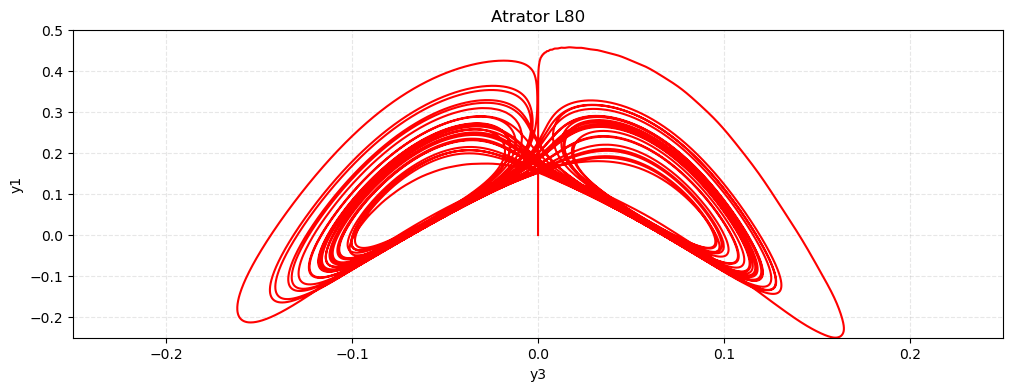
\includegraphics[width=0.7\textwidth]{img/p02y3y1.png}
		\caption{Hadley 01 - Projection $y_3 \times y_1$}
		\label{fig:p02y3y1}
	\end{figure}
\end{frame}

%---------------------------------------------------

\begin{frame}{\textit{PE Model}: Results for Hadley 01 Condition}
	\begin{figure}
		\centering
		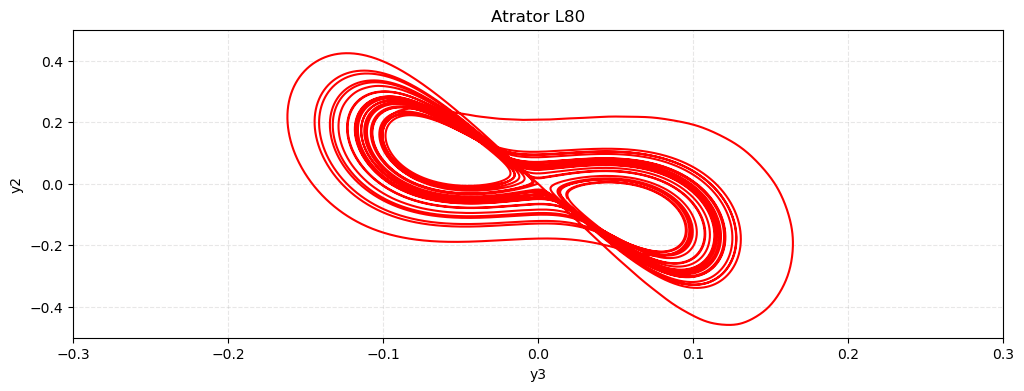
\includegraphics[width=0.7\textwidth]{img/p02y3y2.png}
		\caption{Hadley 01 - Projection $y_3 \times y_2$}
		\label{fig:p02y3y2}
	\end{figure}
\end{frame}

%---------------------------------------------------

\begin{frame}{\textit{PE Model}: Results for Hadley 01 Condition}
	\begin{figure}
		\centering
		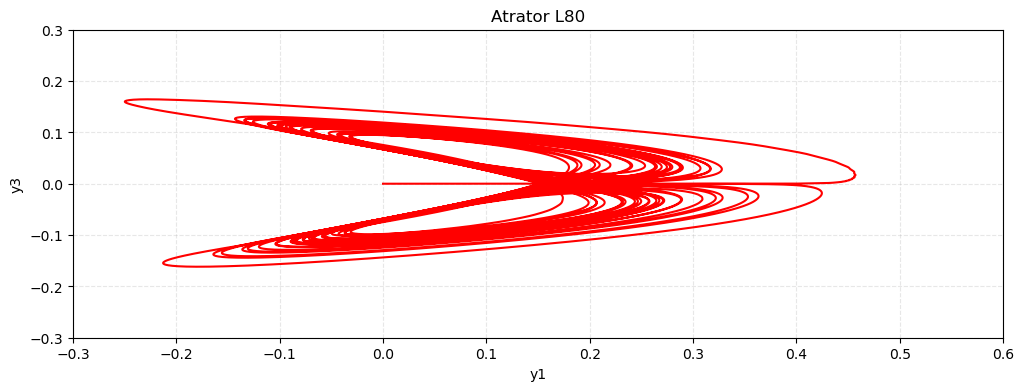
\includegraphics[width=0.7\textwidth]{img/p02y1y3.png}
		\caption{Hadley 01 - Projection $y_1 \times y_3$}
		\label{fig:p02y1y3}
	\end{figure}
\end{frame}

%---------------------------------------------------

\begin{frame}[fragile]
		
	\frametitle{\textit{PE Model and QG Model}: Initial Conditions - Hadley 02}
	The present condition reproduces the Hadley circulation conditions according to \cite{lorenz1980}
	\begin{python}
# Initial conditions of the PE model
hadley02_initial_x = [-0.01111, 0, 0]
hadley02_initial_y = [0.53331, 0, 0]
hadley02_initial_z = [0.53354, 0, 0]
	\end{python}
		
	Equivalent to the following condition in the QG Model:
	\begin{python}
# Initial conditions of the QG model
y0 = [0.53333, 0, 0]
	\end{python}
\end{frame}

%---------------------------------------------------

\begin{frame}{\textit{PE Model} and \textit{QG Model}: Results for Hadley 02 Condition}
	\begin{figure}
		\centering
		\begin{subfigure}[b]{0.45\textwidth}
			\centering
			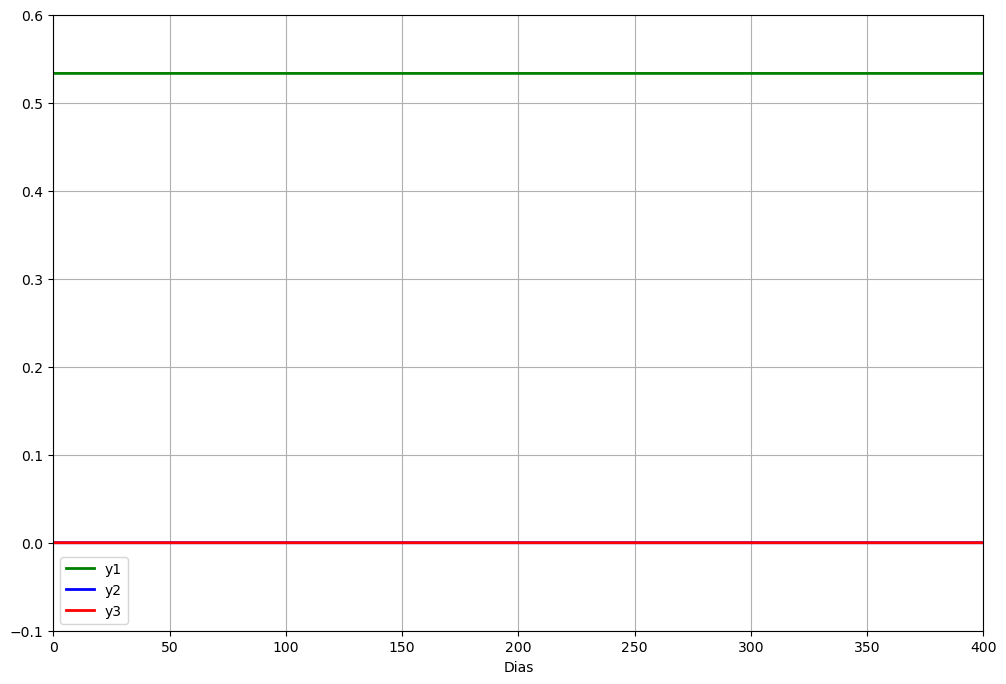
\includegraphics[width=\textwidth]{img/p03d400pe.png}
			\caption{Hadley 02 Condition - 400 days\\ (PE Model)}
			\label{fig:p03d400pe}
		\end{subfigure}
		\hfill
		\begin{subfigure}[b]{0.45\textwidth}
			\centering
			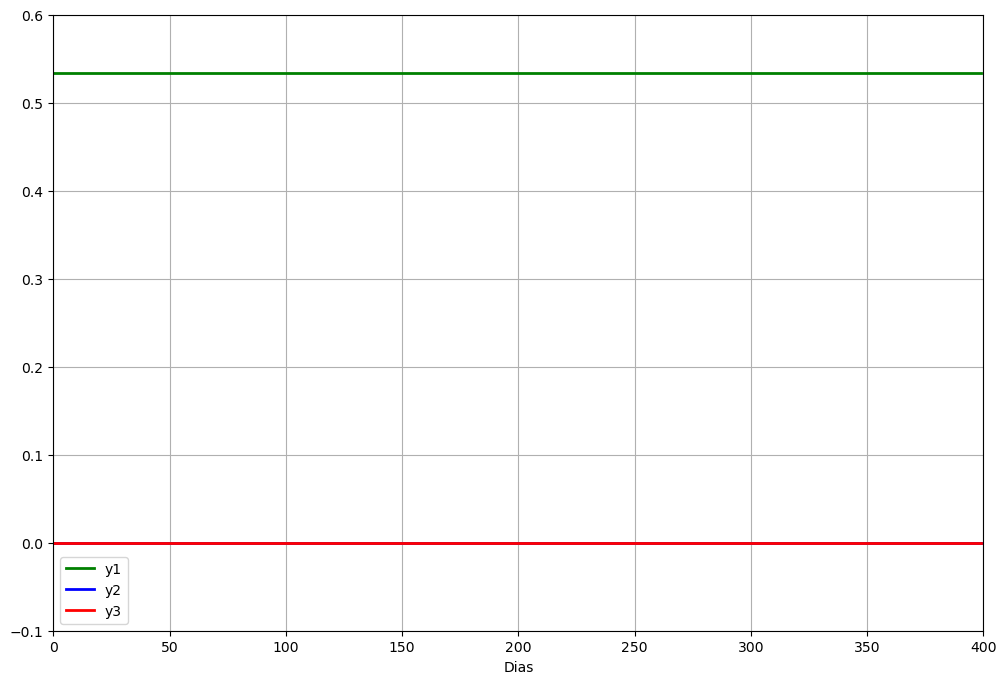
\includegraphics[width=\textwidth]{img/p03d400qg.png}
			\caption{Hadley 02 Condition - 400 days\\ (QG Model)}
			\label{fig:p03d400qg}
		\end{subfigure}
	\end{figure}
\end{frame}

%---------------------------------------------------

\begin{frame}{\textit{Some difficulties}: The equations \eqref{eq:simplified-equation-1}-\eqref{eq:simplified-equation-3}}
		
	\begin{enumerate}
		\item Although equations \eqref{eq:simplified-equation-1}-\eqref{eq:simplified-equation-3} are simplifications of \eqref{eq:primary-equation-1}-\eqref{eq:primary-equation-3}, none of the references used included equations \eqref{eq:simplified-equation-1}-\eqref{eq:simplified-equation-3}.
		\item When attempting to plot \eqref{eq:simplified-equation-1}-\eqref{eq:simplified-equation-3}, several issues arose, the main ones being: \textit{overflow} and deviation from the nature of equations \eqref{eq:primary-equation-1}-\eqref{eq:primary-equation-3}.
	\end{enumerate}
\end{frame}

%---------------------------------------------------

\begin{frame}{\textit{Some difficulties}: The equations \eqref{eq:simplified-equation-1}-\eqref{eq:simplified-equation-3}}
	\begin{figure}
		\centering
		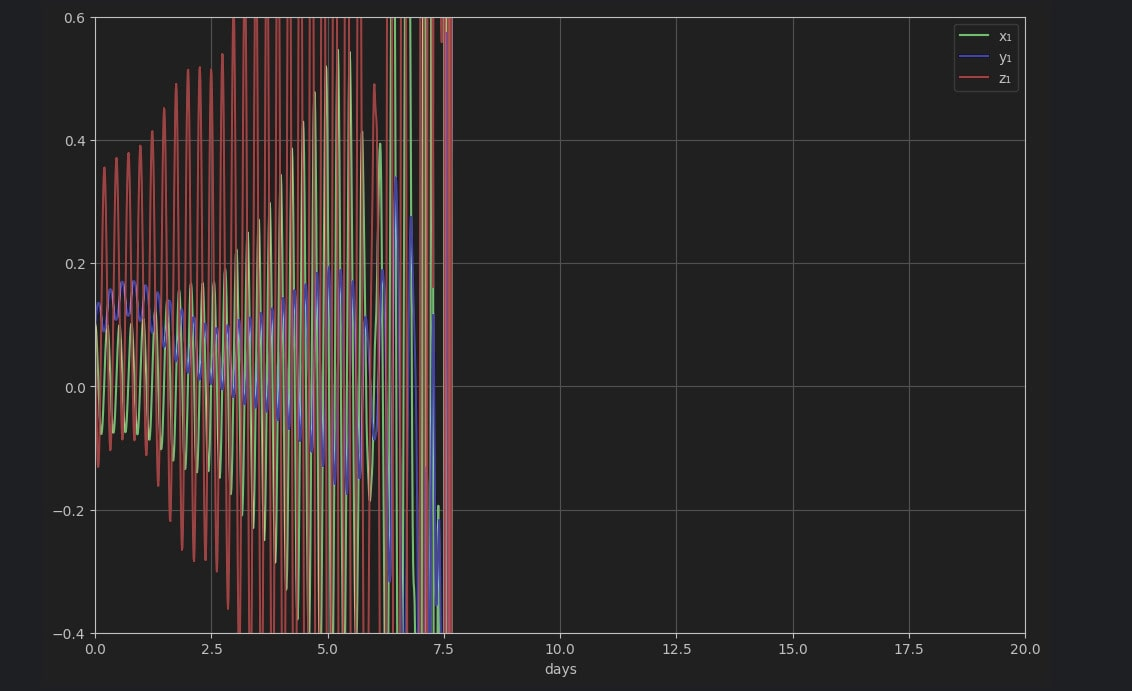
\includegraphics[width=0.5\textwidth]{img/erro_simplificado.jpeg}
		\caption{Attempt to plot equations \eqref{eq:simplified-equation-1}-\eqref{eq:simplified-equation-3}}
		\label{fig:erro-plotagem-eq-simp}
	\end{figure}
\end{frame}

%---------------------------------------------------

\begin{frame}{\textit{Some difficulties}: Equations \eqref{eq:primary-equation-1}-\eqref{eq:primary-equation-3}}
	\begin{figure}
		\centering
		\begin{subfigure}[b]{0.45\textwidth}
			\centering
			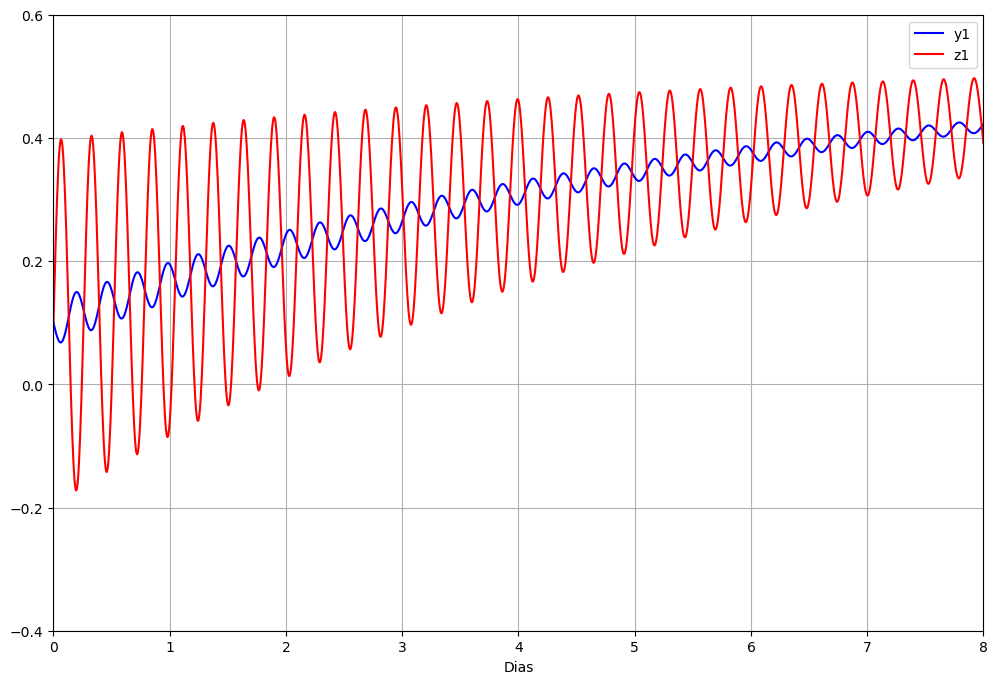
\includegraphics[width=\textwidth]{img/p01d08.png}
			\caption{Standard condition - 8 days}
			\label{fig:p01d08}
		\end{subfigure}
		\hfill
		\begin{subfigure}[b]{0.45\textwidth}
			\centering
			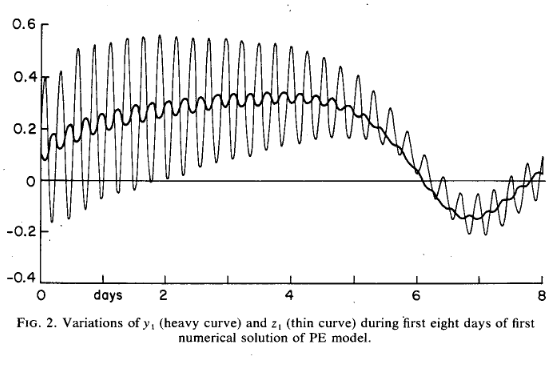
\includegraphics[width=\textwidth]{img/p01d08rel.png}
			\caption{Standard condition - 8 days (article)}
			\label{fig:p01d08rel}
		\end{subfigure}
	\end{figure}
\end{frame}
